\chapter{Problem analysis}

Biomolecular simulations are becoming increasingly important for drug development. In these simulations, force field models are required to describe the interatomic relations of the drug molecules. Often used force field models include \verb|AMBER|, \verb|CHARMM|, \verb|GROMACS|, \verb|GROMOS| and \verb|OPLS|. In order to run a simulation. These force fields require a certain topology. This topology should include the atom types, bonds, angles, atomic charges and charge group assignments.

Figure \ref{fig:partial_charges} shows the topology of a nitroethane molecule. Here, every oval symbolises an atom. The atom type is the letter on the top rule of the oval, i.e. \verb|H| is the atom type of the sphere \verb|H5 (6)|. The first number indicates the index in the list of atoms of that type (\verb|5| in the example), the second the overall atom index in the molecule (\verb|6| in the example). The bonds between atoms are shown as lines between the ovals and the atomic charges are given by the number at the bottom row of the oval (\verb|0.071| for \verb|H5 (6)|). Finally, the colouring of the atoms and the squares around them denote a molecular charge group. These are groups of connected atoms, for which the total charge is ideally equal to that of the whole molecule.

\begin{figure}[h!]
\begin{center}
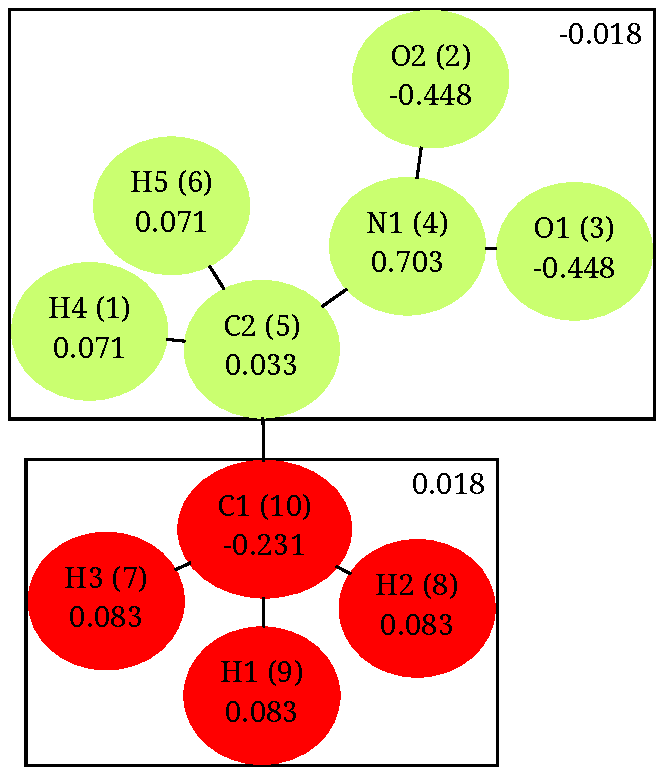
\includegraphics[width=.4\textwidth]{img/partial_charges.pdf}
\caption{Topology of nitroethane ($C_{2}H_{5}NO_{2}$).}
\label{fig:partial_charges}
\end{center}
\end{figure}

In a recent study, El-Kebir, Klau et al. have developed an algorithm that allows for fast and reasonable assignment of charge groups~\cite{canzar2012charge}. As this is now optimized, they focuss on a different step in the parameterization, that of calculating the atomic partial charges. % TODO: etc


Here you present your analysis of the problem situation that your research will address. How does this problem manifest itself at your host organization? Also summarizes existing scientific insight into the problem (result of your literature survey, see below).

\lipsum[5]

